\subsection{Diseño de \texttt{moldeas-common}}\label{sect:moldeas-common}
El objetivo de este módulo es aunar aquella funcionalidad y lógica 
de negocio común a todos los procesos del ciclo de vida. De esta forma y 
atendiendo al modelo de construcción de aplicaciones Java propuesto 
por Maven se pueden separar responsabilidades entre los distintos 
componentes, compilar y empaquetar (como fichero \gls{JAR}) por separado las distintas clases 
de Java de manera transparente.

Entre las funcionalidades entregadas en este paquete hay que destacar 
las siguientes:
\begin{itemize}
 \item Clases para la carga de ontologías y de documentos RDF desde distintas 
fuentes de datos como ficheros o un \textit{endpoint} de \gls{SPARQL}. 

El doble objetivo de diseño de estos paquetes es: 1) independizar la ejecución de los procesos de la base de conocimiento 
y 2) abstraer la localización  (local, remoto, base de datos, etc.) y contenido del recurso.

Para diseñar estos dos objetivos se han seguido los siguientes criterios:
\begin{enumerate}
  \item El patrón \textit{\gls{DAO}} que sirve como guía para este primer objetivo, abstrayendo
  las operaciones necesarias sobre la base de conocimiento a un interfaz que
  pueda ser implementado por distintos proveedores.
  \item El segundo objetivo, se obtiene factorizando la
  información invariante de los recursos: el contenido del recurso puede ser siempre un
  \textit{InputStream} y todo recurso podrá ser localizado por un identificador
  único (nombre fichero, \gls{URL} o un id. de una base datos), no obstante para
  facilitar la abstracción de la clave de un recurso se ha diseñado como un
  objeto (\textit{KnowledgeResourcePK}) anticipando la necesidad de claves más
  complejas que una simple cadena identificativa. 
\end{enumerate}

En la Figura \ref{fig:moldeas-loading}, se realiza un diagrama de clases del módulo de acceso
a la base de conocimiento.

\begin{figure}[!htb]
\centering
	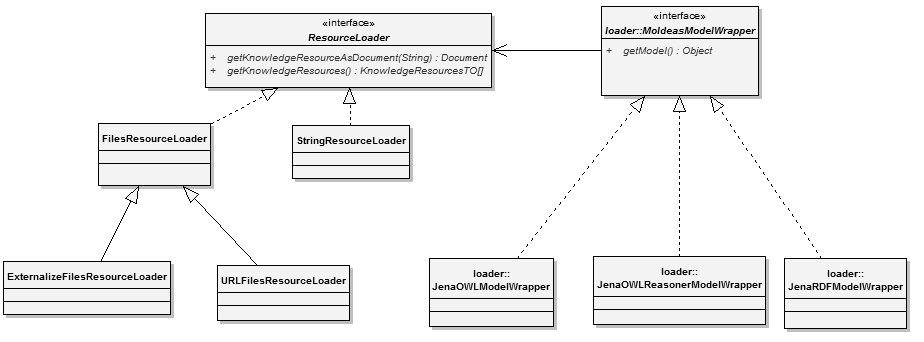
\includegraphics[width=16cm]{images/phd/moldeas/moldeas-loading}
\caption{Diagrama de Clases del acceso a datos (ontologías y RDF) en MOLDEAS.}
\label{fig:moldeas-loading}
\end{figure}


Uno de los puntos clave para facilitar un soporte escalable a los distintos lenguajes y
consiste en la selección del \gls{API} para trabajar con ontologías y recursos RDF. Para ello y teniendo 
en cuenta el uso del lenguaje de ontologías OWL y su representación bajo el modelo 
de datos RDF en sus distintos formatos se debe realizar una abstracción que permita procesar 
la información y los datos con comodidad, ocultando los detalles de representación sintáctica 
y ofreciendo las abstracciones básicas de \gls{OWL} y \gls{RDF}: sentencias, sujeto, recurso, clases, 
propiedades, etc. En este sentido, las alternativas disponibles se centran en:

 \begin{description}    
  \item[Jena:] biblioteca Java de referencia para el trabajo en el 
campo de la Web Semántica conteniendo múltiples funcionalidades para el desarrollo 
de aplicaciones basadas en RDF y OWL. Se trata de \textit{software libre} 
inicialmente desarrollado por \textit{HPLabs} y ahora bajo la fundación Apache.

\item[OWL-API:] es una biblioteca para Java específicamente diseñada para tratar ontologías expresadas en OWL. 
Se distribuye bajo licencia de \textit{software} libre y ha sido creada como parte de proyecto europeo 
\textit{WonderWeb}, en la actualidad es gestionada en la Universidad de Manchester. 

\item [Protégé-OWL-API:] utilizada en el IDE Protégé para el desarrollo de ontologías en OWL. Combina aspectos
 tanto de OWL-API como de Jena. No obstante, su ámbito está más orientado hacia a este editor que como biblioteca 
para un usuario programador.         
\end{description}

Una vez valoradas las posibilidades de estas herramientas, se ha seleccionado Jena y que da soporte 
para el tratamiento de varios lenguajes y formatos de modelado, permite la integración con herramientas 
y procesos externos como los razonadores además de que su comunidad ha crecido exponencialmente 
en los últimos tiempos gracias a su adhesión al proyecto Apache, lo que le confiere un grado 
de madurez y confianza extra que asegura un correcto funcionamiento.


\item Clases para el almacenamiento de constantes a lo largo del ciclo de vida 
de los datos manejados por el sistema \gls{MOLDEAS}. En este sentido, es conveniente parametrizar 
los valores de las \gls{URI}s base, los grafos RDF así como los prefijos y espacios de nombres 
de todos los vocabularios y \datasets reutilizados. Esta práctica evita los errores 
ortográficos en la codificación de URIs tanto en la producción de datos como en su consumo 
a través de consultas SPARQL o mediante el propio API definido por Jena.


\item Clases para la gestión de errores y excepciones que se puedan producir a lo largo de cada uno de los procesos 
del ciclo de vida. 


El diseño de la gestión de errores es uno de los elementos importantes para la
robustez de un producto \textit{software}. Las directrices que se han seguido en MOLDEAS 
para el control de errores es el uso de las excepciones. Para ello, se ha creado 
una simple jerarquía de excepciones que capture los posibles errores dentro de la aplicación. 
Se han considerado dos tipos de excepciones, ver Figura~\ref{fig:diagramas/excepciones}:
\begin{description}
\item[Excepciones no chequeadas:]  controlan errores graves producidos en tiempo
de ejecución e inesperados en el modelo. 
\item[Excepciones chequeadas:] controlan errores graves que se pueden producir
en tiempo de ejecución y de los cuales la aplicación se puede recuperar. 
\end{description}


\begin{figure}[htb]
\centering
	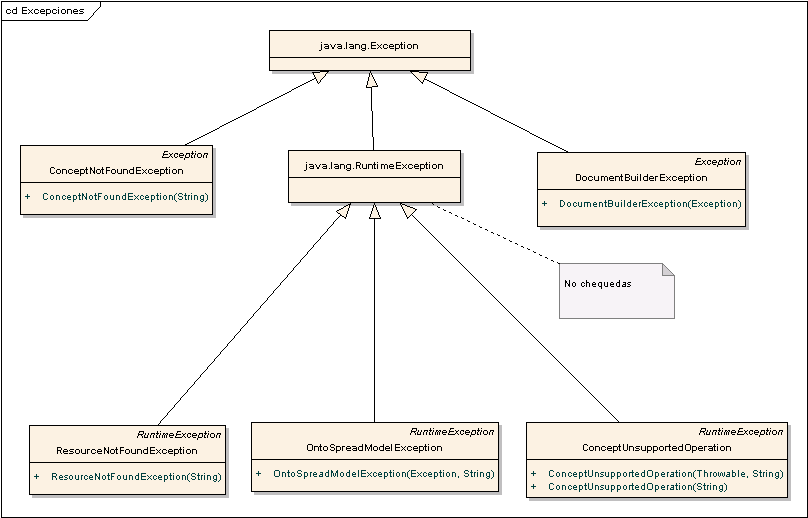
\includegraphics[width=16cm]{images/phd/moldeas/excepciones}
\caption{Diagrama Clases de excepciones en el sistema MOLDEAS.}
\label{fig:diagramas/excepciones}
\end{figure}

\item Clase para la configuración del registro y traza de la aplicación. 

Esta característica de verdadero valor para una aplicación permite agilizar los procesos de depuración y su integración 
en sistemas de mayor calado. En todas las clases del sistema MOLDEAS, candidatas a 
generar mensajes de registro se ha utilizado la biblioteca \textit{Log4j} 
para la gestión del registro de la aplicación. Se trata de una herramienta 
Java para la gestión del registro y traza de acuerdo a un serie de 
niveles: \textit{DEBUG, INFO, WARN, ERROR y FATAL}. Esta división por niveles 
permite configurar los mensajes del sistema dependiendo del estado 
en el que se encuentre: desarrollo, depuración, producción, etc.

La configuración de este registro se realiza mediante la carga 
de un fichero XML o \textit{properties} de Java en el cual se especifica el nivel antes comentado 
a través de una serie de propiedades y para cada uno de los paquetes 
de la aplicación. Así, los tres elementos básicos a definir son: \textit{Appenders} (dónde 
se van a escribir los mensajes de registro), \textit{Layouts} (cómo se van a escribir, formato) y \textit{Loggers} (quién 
los va a escribir). Log4j permite definir para cada clase o paquete, las propiedades de su
\textit{logger}, es decir, su \textit{layout} y \textit{appender}, con solicitar
para una determinada un \textit{logger} (instancia de \textit{Logger}) ya se puede utilizar la
biblioteca de registro. El uso de esta biblioteca está perfectamente demostrado, 
ya que son muchas las aplicaciones Java que utilizan Log4j para dar soporte este tipo de tareas.


\item Otras clases de utilidad para acciones transversales como la carga de documentos 
\gls{XML}, ejecución de consultas \gls{SPARQL}, filtros de lenguaje natural para las bibliotecas 
de Apache \gls{Lucene} y \gls{Solr}.

\end{itemize}

\subsection{Diseño de \texttt{moldeas-transformer}}\label{sect:moldeas-transformer}
El objetivo de este módulo es facilitar el soporte al proceso específico 
de producción de datos enlazados para las distintas entidades de información 
provenientes de los anuncios de licitación. En el enfoque de este trabajo 
se ha tenido en cuenta los datos a transformar y promocionar a la iniciativa 
de \linkeddata para agilizar las distintas tareas del modelo de ciclo 
de vida de datos enlazados propuestos. Existen ciertas tareas 
que se pueden acometer directamente con las herramientas existentes como 
Google \gls{Refine} y que su funcionamiento es correcto cuando 
los datos son homogéneos y tan sólo requieren la ejecución de una serie 
de \textit{mapeos} o reglas de transformación para utilizar los datos 
de entrada como valores en las tripletas \gls{RDF} a generar. Sin embargo, 
dependiendo del tamaño del \dataset de entrada a transformar, de la homogeneidad 
de los mismos y de las operaciones posteriores a realizar como la adición de metainformación, 
la reconciliación de entidades o la simple serialización del modelo RDF en distintos 
formatos, hace necesario la implementación de un proceso personalizado que ejecute 
estas tareas de forma específica ya que la dificultad de expresarlas en las herramientas 
de propósito general las hace tremendamente complicadas. Es por ello, que se ha diseñado 
e implementado en este módulo una serie de funcionalidades de carácter específico 
para cada una de las entidades a transformar teniendo presente las características 
de las mismas. Para ello, se han considerado los siguientes puntos:

\begin{itemize}
 \item La transformación de la información propia de los anuncios de licitación conlleva la promoción 
de una gran cantidad de datos que pueden ser tomados de distintas fuentes 
como fichero \gls{CSV}, MSExcel, \gls{XML} o desde una base de datos. En este sentido, 
y debido a dos variables importantes como son el tamaño del \dataset y la diversidad 
de los formatos de entrada se ha optado por la implementación de una serie de adaptadores 
que permiten procesar la información de entrada de forma homogénea para que la generación 
en RDF se convierte en un proceso transparente de la fuente de datos y se pueda asegurar 
la validez de los datos transformados. En cuanto a la reconciliación de entidades para este 
conjunto de datos no se considera necesaria ya que se realiza específicamente en el catálogo 
de clasificaciones de productos, sin embardo el enriquecimiento del \dataset de entrada si 
se ve afectado ya que se han añadido nuevas propiedades (latitud y longitud) a los códigos NUTS para facilitar 
posteriores procesos como el de búsqueda de anuncios de licitación. 

Por tanto, los anuncios de licitación se transforman mediante un proceso Java \textit{ad-hoc} que cubre 
todas las tareas del ciclo de vida referentes a la producción de datos enlazados.

\item En cuanto al catálogo de clasificaciones y teniendo en cuenta las características de las mismas: 
tamaño relativamente pequeño y formato de entrada homogéneo, se ha optado por un enfoque híbrido, en el cual 
en el primer paso se realiza la transformación de los datos originales mediante la herramienta Google 
Refine para una vez obtenidos los datos en RDF realizar una serie de pasos específicos para la 
reconciliación de entidades (enlazado de las distintas clasificaciones con el CPV 2008) y la adición 
de metainformación. Para ello, se ha implementado un proceso Java capaz de tomar como fuente de datos 
RDF e ir accediendo y enriqueciendo cada una de las descripciones de productos y servicios disponibles, 
basándose en la construcción de un reconciliador de entidades específico con las bibliotecas de 
Apache \textit{Lucene} y \textit{Solr}.


\item Por último y en los datos particulares de organizaciones, países y personas se ha utilizado 
de nuevo un enfoque híbrido en el cual para la transformación inicial se ha optado por la herramienta 
de Google Refine, enriqueciendo y añadiendo a los datos RDF ya generados las tripletas de información 
necesarias para cumplir con la especificación de recursos RDF realizada.

\end{itemize}

En general, este módulo consta de una serie de procesos independientes que son capaces para cada una 
de las grandes entidades de información provenientes de los anuncios de licitación públicos de procesar 
los datos en distintos formatos, realizar el proceso de reconciliación de entidades y enriquecer los 
\datasets de entrada mediante la adición de metainformación. 


\subsection{Diseño de \texttt{moldeas-api}}\label{sect:moldeas-api}
Atendiendo a las consideraciones generales sobre diseño, se explicarán 
las decisiones de diseño más relevantes para la construcción 
de un \gls{API} que provee los métodos necesarios para el consumo de datos 
enlazados provenientes de la información de los anuncios de licitación, 
incluyendo las clasificaciones de productos, países y organizaciones.

Este módulo del sistema \gls{MOLDEAS} se encarga de entregar la funcionalidad 
básica, a través de un fichero \gls{JAR}, para dar soporte a los siguientes servicios:
\begin{itemize}
 \item Consumo de los datos enlazados provenientes de los anuncios de licitación, 
clasificaciones de productos y organizaciones desde un entorno de programación y, 
en este caso, desde el lenguaje Java.
\item Construcción de un sistema de recuperación de información que sea capaz de generar 
consultas en \gls{SPARQL} para ser ejecutadas en el \textit{endpoint} en el cual se encuentran 
almacenados todos los datos.
\end{itemize}

Para dar soporte a estos dos grandes servicios se han establecido una serie de paquetes, 
ver Figura~\ref{fig:moldeas-api-packages}, en los cuales se realizan las funciones 
necesarias que permiten la ejecución de estos servicios. En este dimensionado por paquetes 
se establecen las siguientes funcionalidades:

\begin{itemize}
 \item El paquete \texttt{dao} en el cual se encuentran las interfaces 
que definen las operaciones necesarias para el acceso a los datos enlazados 
de los anuncios de licitación.

\item El paquete \texttt{impl} en el cual se implementan las interfaces 
anteriores mediante clases que realizan el \textit{mapeo} real 
desde los objetos Java de lógica de negocio a los datos enlazados 
que se encuentran en un \dataset RDF. En este caso, los datos se cargan a través 
de consultas en SPARQL que se pueden ejecutar contra un modelo RDF en memoria 
o bien remotamente en un \textit{endpoint}. El objetivo de este paquete es proveer 
la carga de objetos Java con los datos enlazados provenientes de los anuncios de licitación, 
por ello para cada una de las entidades identificadas se suministra un interfaz de acceso 
que genera las consultas en SPARQL adecuadas para extraer los datos del \dataset RDF. Este 
paquete constituye por tanto el nivel de acceso primario y básico a los datos enlazados 
constituyendo la primera capa de lógica y acceso a datos del sistema MOLDEAS. Como ejemplo 
se presenta el acceso a datos para los códigos CPV mediante un diagrama de clases, 
ver Figura~\ref{fig:moldeas-api-dao}.

\begin{figure}[!htb]
\centering
	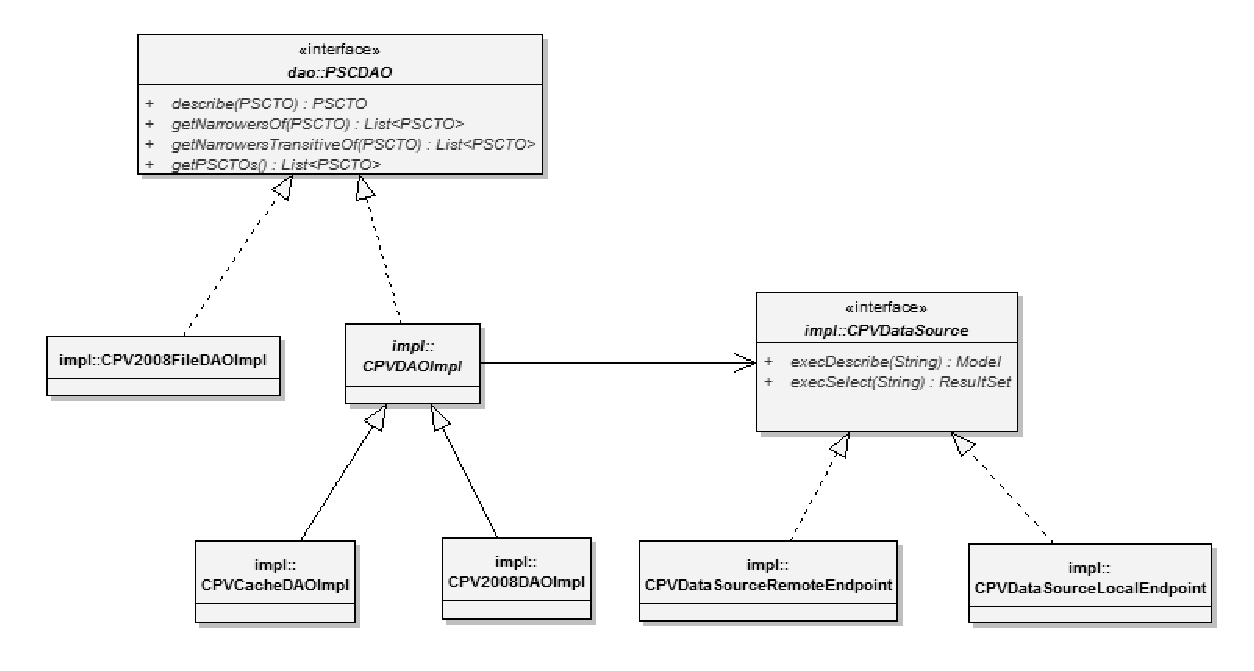
\includegraphics[width=16cm]{images/phd/moldeas/moldeas-dao}
\caption{Diagrama de Clases del acceso a datos (CPV) en \texttt{moldeas-api}.}
\label{fig:moldeas-api-dao}
\end{figure}


\item El paquete \texttt{appserv} en el cual se encuentran las clases con los servicios 
de negocio propios del sistema MOLDEAS, principalmente el servicio de recuperación 
de información y construcción de consultas en SPARQL a partir de un perfil de búsqueda 
del usuario. Adicionalmente, se encuentran clases relativas a la gestión de los objetos 
con la información de los anuncios de licitación.

\item  El paquete \texttt{enhancers} en el cual se establecen las interfaces para la 
expansión de las variables de información correspondientes a un perfil de búsqueda 
de anuncios de licitación. Entre los métodos especificados para realizar la expansión 
de consultas se encuentran aquellos relativos a \textit{Spreading Activation} a través 
de la biblioteca ONTOSPREAD, los basados en un motor de recomendación como Apache Mahout,
 los basados en un motor de búsqueda sintáctica como Apache Lucene y los relativos 
a las variables numéricas. 

\item El paquete \texttt{psc} en el cual se implementan las interfaces específicas relativas 
a la expansión de la variable de información de los anuncios de licitación correspondiente 
a las códigos de una clasificación de productos, en concreto del CPV 2008. Los métodos aquí 
utilizados son los relativos a la aplicación y configuración de las bibliotecas ONTOSPREAD, 
Apache Mahout, Lucene y Solr.

\item El paquete \texttt{standalone} en el cual se implementan las interfaces específicas 
para otras variables de información secundarias como la información geográfica o la cuantía 
del anuncio de licitación, en este caso de nuevo el principal componente utilizado es la biblioteca 
Apache Mahout configurada a través de distintos ficheros generados mediante el análisis 
del histórico de publicación de anuncios de licitación. Cada una de las implementaciones 
dependiendo de la información que se pretenda manejar debe tomar sus datos en un tabla 
previamente generada en el módulo de \texttt{moldeas-transformer}.

\item El paquete \texttt{ranking} en el cual se específica y se realiza una primera implementación 
de los operadores de agregación para establecer un orden los anuncios de licitación recuperados 
del \dataset RDF, ya sea través de un modelo en memoria o de un \textit{endpoint} de SPARQL. Para cada 
una de las variables de información presentes en los anuncios de licitación se estable un peso, cuando 
los anuncios de licitación son recuperados tras el proceso de expansión se establece una puntuación 
mediante una función lineal que establece un valor según el anuncio extraído contenga más o menos 
elementos de los conjuntos relativos a los códigos \gls{CPV}, \gls{NUTS}, etc.

\item El paquete \texttt{business} establece el interfaz de negocio para interactuar con los servicios 
del API, de esta manera se suministra un único punto de acceso como una caja negra favoreciendo la 
abstracción del número de parámetros y las operaciones.
\end{itemize}

\begin{figure}[!htb]
\centering
	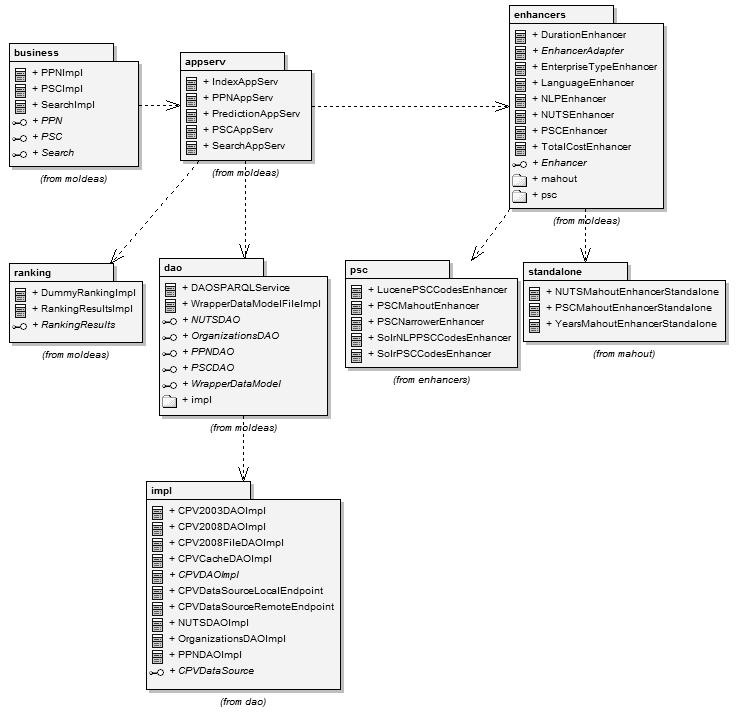
\includegraphics[width=16cm]{images/phd/moldeas/moldeas-api-packages}
\caption{Diagrama de Paquetes relevantes del componente \texttt{moldeas-api}.}
\label{fig:moldeas-api-packages}
\end{figure}

Una vez revisados los principales paquetes de \texttt{moldeas-api} cabe realizar una descripción 
más completa del sistema de recuperación de información ya que el sistema de expansión de consultas 
se implementa a través de un patrón de diseño denominada \texttt{Chain of Responsibiliy} en el cual 
a través de distintas iteraciones y modificaciones de la consulta inicial se consigue un perfil 
enriquecido para ser traducido a una consulta en SPARQL. Evidentemente, el objeto contenedor 
del perfil de búsqueda de anuncios de licitación puede ser transformado a cualquier lenguaje de 
consulta tipo SQL o bien a una consulta de un motor de búsqueda sintáctica, esta abstracción 
se consigue de nuevo gracias a un uso correcto de interfaces. En primer lugar cabe especificar 
qué tipo de información y datos contiene un anuncio de licitación que como ya se ha repasado en 
el Capítulo~\ref{capitulo:metodos-separados} y más en concreto en la Sección~\ref{sect:rdf-anuncios} consta 
de una serie de variables de información conteniendo códigos del tipo de licitación, información geográfica, 
metainformación relativa a la cuantía del contrato, el perfil del contrante, la duración, etc. En general, 
y de acuerdo a la información disponible y su tipo se pueden establecer una serie de métodos para realizar la expansión 
de una consulta o perfil de búsqueda.

\begin{itemize}
 \item Información basada en conjuntos y modelada a través de una jerarquía. Se trata el caso de los códigos CPV y de la información 
geográfica disponible en NUTS. En este caso los métodos que se pueden aplicar para expandir la consulta son los siguientes:
\begin{enumerate}
 \item Directo. Se navega a través de la jerarquía modelada buscando los elementos más específicos y estableciendo 
un peso determinado para cada uno de los elementos más específicos. 
 \item Búsqueda Sintáctica. De acuerdo a las descripciones de los códigos se realiza una búsqueda en el \dataset correspondiente 
buscando no sólo aquellos códigos que encajen perfectamente sino también los que son similares mediante técnicas de procesamiento 
de lenguaje natural.
\item Motor de Recomendación. Realizando un procesamiento previo del histórico de anuncios de licitación y su información se generan 
una serie de ficheros en los cuales se alinean los códigos CPV con la información relativa a la localización, cuantía o fecha, para que 
de acuerdo a una serie de códigos de entrada se generen una serie de información de salida.
\item \texttt{Spreading Activation}. En este caso se configura esta técnica para que tome un conjunto de conceptos de entrada, en general 
de códigos CPV, para obtener tras la ejecución del algoritmo un conjunto de salida ponderado.
\end{enumerate}

\item Información numérica o asimilable. Se trata el caso de la duración del contrato, la cuantía del mismo, 
el radio de acción geográfico, etc. En este caso los métodos que se pueden aplicar para expandir la consulta son los siguientes:
\begin{enumerate}
\item Basado en el usuario. El perfil búsqueda del propio usuario define los rangos en los cuales se debe hallar una variable 
numérica sin necesidad de realizar ningún proceso de expansión automático.
\item Uso de lógica borrosa. Se ha valorado el uso de estas técnicas para establecer un intervalo en el cual poder ponderar 
la pertenencia de un valor a un conjunto. No obstante, en esta primera del demostrador público estas técnicas implementadas 
a través de la biblioteca \textit{JFuzzyLogic} tan sólo se han probado y no se han introducido como parte del proceso de 
búsqueda.
\end{enumerate}

\end{itemize}

El objetivo final de estos métodos es obtener para cada una de las variables de información de un perfil 
de anuncio de licitación una puntuación que permite ejecutar un operador de agregación para así establecer 
un orden entre los anuncios de licitación extraídos tras la generación de la consulta. La importancia de este 
procedimiento por fases reside en que cada uno de los pasos y métodos de expansión se modelan mediante interfaces y 
son ejecutados mediante un proceso iterativo de enriquecimiento, como se puede ver en la Figura~\ref{images/phd/moldeas/moldeas-chain}, 
que permite la adición de nuevos métodos de forma sencilla, simplemente reconfigurando las implementaciones de 
los interfaces a través del fichero de configuración de Spring. El flujo y la comunicación 
entre las distintas clases que intervienen en el proceso de expansión y recuperación de información 
se presenta a través de la Figura~\ref{fig:moldeas-api-search}, en el cual es preciso señalar 
como las responsabilidades son compartidas a través de las distintos objetos situados en distintas 
capas lógicas.

\begin{figure}[!htb]
\centering
	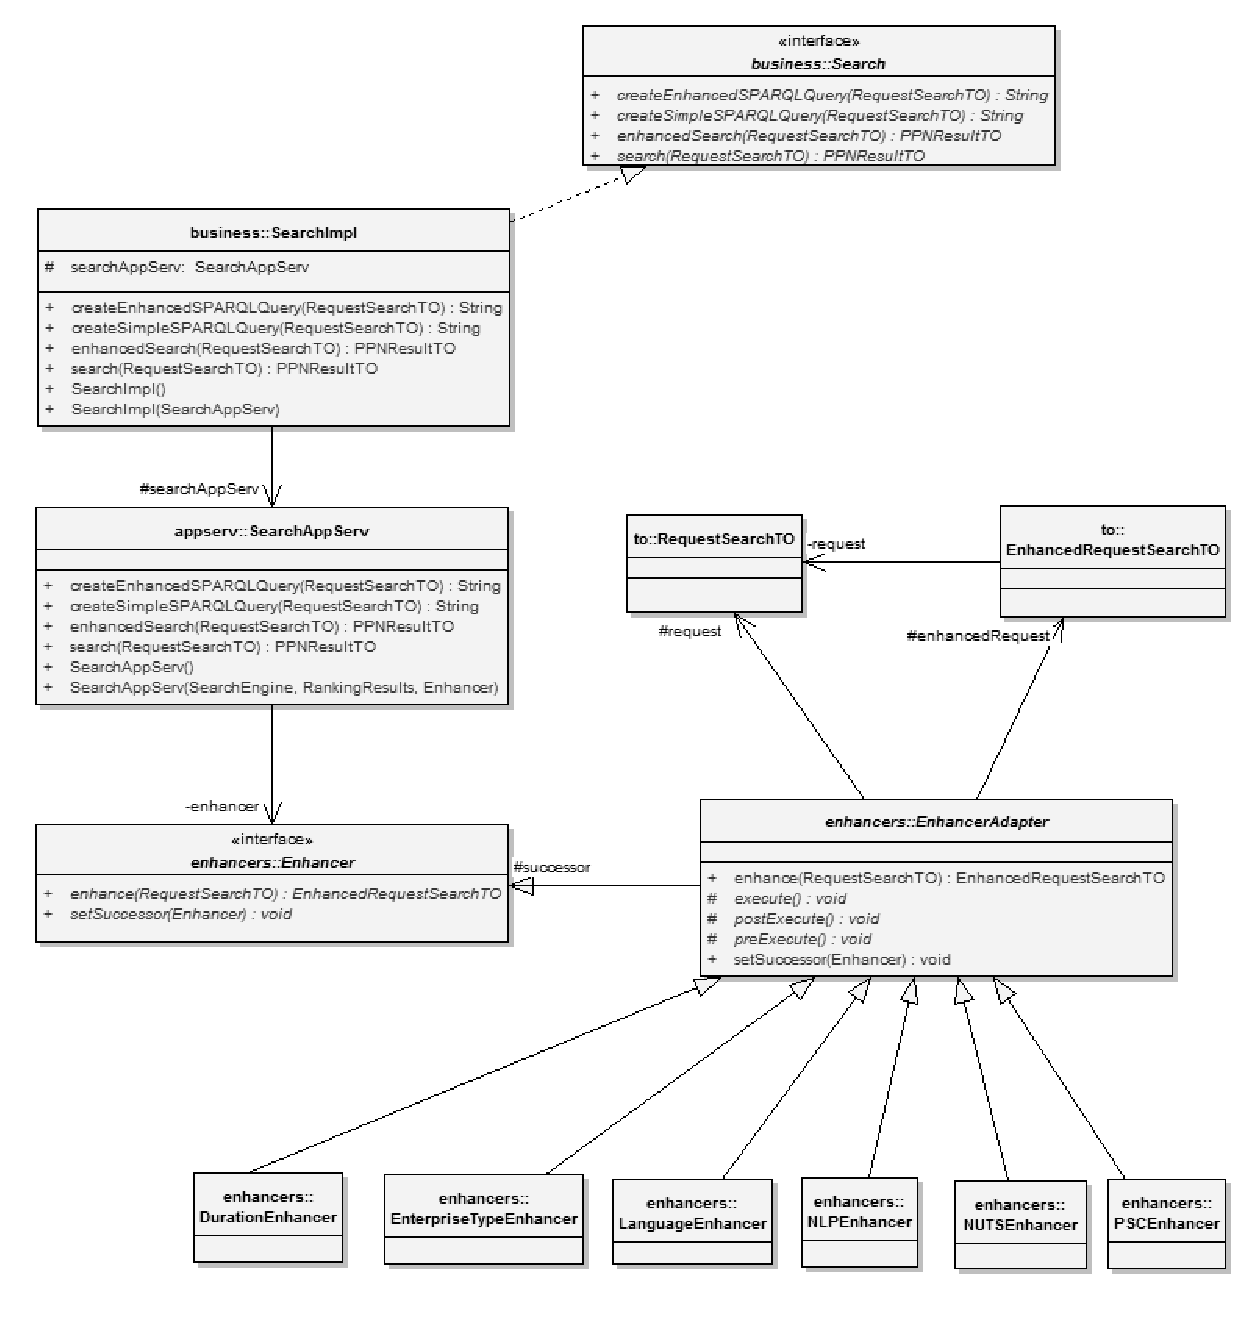
\includegraphics[width=16cm]{images/phd/moldeas/moldeas-chain}
\caption{Diagrama de Clases del sistema de búsqueda en \texttt{moldeas-api}.}
\label{fig:moldeas-api-search}
\end{figure}


\begin{figure}[!htb]
\centering
	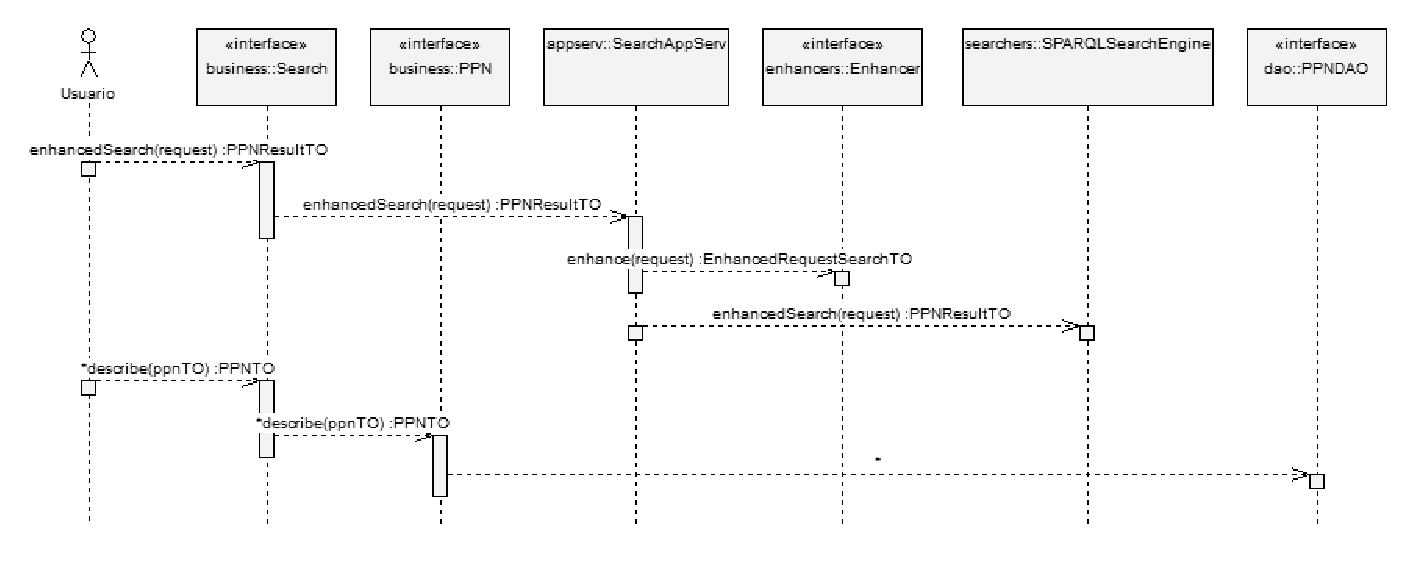
\includegraphics[width=16cm]{images/phd/moldeas/moldeas-search}
\caption{Diagrama de Secuencia de la búsqueda en \texttt{moldeas-api}.}
\label{fig:moldeas-search}
\end{figure}


Finalmente, en este apartado cabe señalar los patrones de diseño, ver Tabla~\ref{tabla:patrones}, que se han aplicado 
para obtener un sistema flexible y escalable en el cual nuevas implementaciones 
de los interfaces sean fácilmente integrables proporcionando un API para la 
el consumo de datos enlazados y recuperación de información de los anuncios de 
licitación.


\begin{table}[htb]
\renewcommand{\arraystretch}{1.3}
\begin{center}
\begin{tabular}{|p{6cm}|p{8cm}|}
\hline
        \multicolumn{2}{|c|}{\textbf{Patrones de Diseño}}\\        
        \hline
        \textbf{Nombre} &  \textbf{Aplicación} \\ \hline       
			\textit{Adapter}&Implementación para el acceso y transformación de los datos de los anuncios de licitación.\\ \hline
			\textit{Chain of Responsibility}&Implantación del sistema de enriquecimiento de consultas.\\ \hline
			\textit{DAO}&Abstracción de acceso a la base de datos y de conocimiento.\\ \hline
			\textit{Template Method}& Implementación por omisión de métodos en el patrón \textit{Chain of Responsibility}.\\ \hline
			\textit{Factory Method}&Creación de objetos provenientes de Spring.\\ \hline
			\textit{Template Method}&Funciones con llamadas a métodos de interfaces, por ejemplo en los \texttt{Enhancers}.\\ \hline
			\textit{Transfer Object}&Comunicación de información entre los distintos módulos y capas.\\\hline 
			\textit{Singleton}&Creación de objetos de acceso a datos, etc. provenientes de Spring.\\ \hline
			\textit{Otros}&Relativos al diseño por capas de aplicaciones J2EE.\\ \hline
		\hline
		\end{tabular}
		\caption{Principales Patrones de Diseño utilizados en MOLDEAS.}
		\label{tabla:patrones}
  \end{center}
\end{table} 

\subsection{Diseño de \texttt{moldeas-test}}\label{sect:moldeas-test}
El objetivo de este módulo es abstraer las pruebas de los módulos anteriores, 
especialmente de \texttt{moldeas-api}, para así proveer un sistema separado 
de ejecución de \textit{tests} en el cual se puedan realizar las siguientes 
acciones:

\begin{itemize}
 \item Creación de configuraciones del \gls{API} de \gls{MOLDEAS} a través de distintos 
ficheros de Spring que permiten probar de forma automática la combinación 
de los distintos métodos de expansión de consultas así como verificar 
sus resultas.
\item Validación de los recursos \gls{RDF} generados de acuerdo a unas reglas de validación 
extraídas de las tablas de validación establecidas en el Apéndice~\ref{tablas-validacion-apen}.
\end{itemize}

De esta manera se ofrece un módulo separado con un doble sentido para la realización de pruebas de caja negra para los 
servicios disponibles en el API de MOLDEAS así como para la propia validación de los datos enlazados. La configuración 
de este módulo se realiza a través de un fichero \gls{XML} \textit{ad-hoc} en el cual se cargan las configuraciones 
para ejecutar los \textit{tests} pertinentes (en forma de plantilla) que se encuentran programas como 
pruebas de Junit. No obstante, en la Sección~\ref{sect:pruebas-moldeas} se realiza una descripción 
más detallada de las pruebas llevadas a cabo.


\subsection{Diseño de \texttt{moldeas-web}}\label{sect:moldeas-web}
El objetivo principal de diseño de este módulo es definir y diseñar un herramienta de acceso gráfico 
a los servicios del sistema \gls{MOLDEAS}. Es importante destacar que este cliente gráfico se realiza con el objetivo de facilitar 
un demostrador público ya que el uso de la biblioteca de \texttt{moldeas-api} es perfectamente 
válido desde cualquier programa así como desde el interfaz de servicios REST, que también se incluye 
en este módulo. Por tanto, este módulo surge para abarcar las siguientes funcionalidades:

\begin{enumerate}
\item Proveer un interfaz de servicios \gls{REST} que sirva tanto para exponer los 
servicios de negocio como para ejemplificar las llamadas del \gls{API} de MOLDEAS.

El interfaz de servicios REST diseñado simplemente añade una capa extra de indirección a los 
servicios de negocio suministrados en el API de MOLDEAS, se duplica la signatura de los métodos 
en una nueva capa simplificando las llamadas. La idea de realizar un interfaz REST surge para dar soporte a la tendencia actual de publicación 
de servicios web \gls{HTTP} y también para ejemplificar las llamadas al API (construcción de parámetros, gestión 
de los resultados, etc.), en cualquier caso, cualquier cliente siempre puede utilizar 
la versión de \texttt{moldeas-api} empaquetada individualmente. Para realizar este API de servicios 
REST se ha utilizado la biblioteca para Java-Jersey \gls{REST} 0.8 y la descripción de los mismos 
se presenta, parcialmente, en la Figura~\ref{fig:moldeas-wadl} en formato \gls{WADL}.


\begin{figure}[!htp]
\lstinputlisting{examples/moldeas-pretty.wadl}
	\caption{Interfaz REST en formato WADL.}
	\label{fig:moldeas-wadl}
\end{figure}


\item Suministrar un interfaz gráfico que ejemplifique las llamadas a los servicios REST y 
a la vez sirva como demostrador público para el acceso a los datos de los anuncios de licitación 
y para la recuperación de información. La construcción de este interfaz se ha desarrollado utilizando 
bibliotecas de Jquery y HTML facilitando la creación de interfaces enriquecidos de programación 
sencilla.

\item Aunar las herramientas externas de publicación y acceso a datos enlazados en un sólo punto de entrada. En este sentido, 
el interfaz web creado también contempla ejemplos de consultas en SPARQL a realizar mediante la herramienta 
\gls{SNORQL} y enlaces a ejemplos de recursos que son consultados a través de un \linkeddata \textit{front-end} como 
Pubby, facilitando tanto el acceso al sistema de recuperación de información como el consumo directo 
de datos enlazados mediante la navegación tradicional.

\end{enumerate}

\subsubsection{Conceptos y Diseño de la Interacción Gráfica}
En los últimos años, el aumento en el uso de las nuevas tecnologías de la información ha 
conllevado un cambio fundamental en la sociedad que provoca la necesidad de adecuarnos a nuevas 
relaciones que se establecen entre la persona y la máquina. Esta necesidad de interacción sugiere 
que la comunicación persona y máquina adquiera una especial relevancia en nuestro tiempo. Todo esto 
propone un desafío consistente en dotar de significado a los productos y servicios ofrecidos, 
intentando dotarlos de estructura y comprensión cercana a la escala humana.

Debido a la complejidad interna de los ordenadores, la comunicación entre los entes debe realizarse 
a un nivel conceptual, predominando la comunicación visual, gráfica y verbal como medio para llegar 
a la comprensión. La idea que subyace reside en encontrar el modelo ideal que permita a la persona 
interaccionar con las máquinas como si fueran un humano más.

En esta situación se hace especialmente relevante la generación de interfaces de usuario 
que se adecuen a las necesidades de las personas, por ello las reglas propuestas por 
\textit{Sneiderman} suponen un primer acercamiento a la interacción persona ordenador y una 
métrica para evaluar la bondad de un interfaz de usuario.

En este sentido, desde el principio de la historia los hombres han ideado formas e instrumentos
(lenguajes de símbolos, de texto, gráficos, etc.), para la comunicación de sus experiencias, 
como para reproducir la realidad. La forma de expresión depende en buena medida del ambiente 
tecnológico y de los lenguajes utilizados entre el emisor y el intérprete para decodificar los mensajes. 

La riqueza de expresión de un lenguaje se basa en el principio de concordancia entre los entes 
participantes del acto comunicativo. Para que se establezca este acto deben estar en correcta relación. 
Desde el punto de vista de un interfaz gráfico estos factores quedan patentes por la dificultad 
que entraña ofrecer un entorno en el cual tanto: percepción, interpretación y comprensión sean 
lo suficientemente claros para que la persona humana no se sienta en un entorno extraño.

En el caso de los seres humanos, mediante el sistema nervioso somos capaces de percibir todo lo ocurre en nuestro 
entorno y actuar en consecuencia. Se puede considerar que el hombre es una fuente de información 
por la cual la información fluye, percibimos y recibimos estímulos externos que nos permiten 
adaptar nuestras respuestas. 

Enorme dificultad supone entender el comportamiento humano como sistema de comunicación, 
tanto en capacidad para interpretar, como para decodificar los mensajes, haciendo imposible 
conocer su respuesta exacta ante la recepción de un mensaje. El problema de la comunicación entre personas y 
máquinas no consiste en reducir el comportamiento humano al de una máquina, sino analizar 
las necesidades y capacidades para adaptar la presentación de información a su nivel 
y acercarnos lo más posible al proceso cognitivo de la persona.

La visión es nuestro medio natural de percepción de los mensajes, limitada por condiciones físicas, 
por ello cobra especial relevancia a la hora de la distribución de información en un documento, 
dependiendo la compresión de la persona de la bondad de esta distribución. No obstante, este modelo a seguir no es 
completamente válido ya que habría que tener en cuenta las necesidades de las personas con discapacidades de distinto tipo, 
intentado adaptar el contenido al sujeto participante de la comunicación.

Utilizando los distintos sentidos de los que disponemos como fuentes de adquisición de información 
debemos ser capaces de procesar y comprender esta información, esta capacidad la podemos denominar 
\textit{entendimiento humano}, mediante el cual determinamos nuestros actos a partir de las percepciones 
sensoriales. De todos estímulos que percibimos, sólo nos quedamos con aquellos que nos impactan más, 
este será un factor muy relevante a la hora de diseñar un interfaz por ejemplo cuando seleccionamos 
una combinación de colores.

Debemos tener en cuenta, que aunque el funcionamiento general humano es similar no puede ser 
predecible y ni aplicable a todo el mundo por extensión, se caería en un grave error de 
interpretación del comportamiento, este punto es especialmente interesante a la hora de adaptar un interfaz 
gráfico a las distintas personas, estableciendo perfiles.

Las 8 reglas de Oro de \textit{Sneiderman} nos ayudan a este objetivo, intentando simplificar 
la comunicación persona-máquina. A continuación, se comentan estas reglas.

\begin{description}
\item[Esforzarse por la consistencia.] Es el principio por el cual los
elementos, relaciones deben ser presentados de forma idéntica e inequívocamente.

Este concepto es aplicable a:
\begin{itemize}
\item Tipografía, por ejemplo enfatizar siempre con el mismo estilo.
\item Iconos, la misma acción debe estar representada por el mismo icono.
\item Comandos y menús, la información que se utilice en los menús deberá ser representativa
de su acción interna.
\item Funcionamiento multiplataforma, esta cualidad se pone muy de manifiesto hoy en día, ya que la misma información es accedida utilizando diferentes medios: navegadores, móviles, pda's, etc.
\item Percepción del sistema igual para todos los usuarios.
\item Estructura el sistema de forma que se adapten al entorno de trabajo del usuario.
\end{itemize}

Por lo tanto la consistencia nos remite a obtener una representación de los objetos 
coherente en su significado, formas y métodos en el mismo contexto. 
También podemos entender la consistencia como la relación que se establece entre 
una metáfora de representación y su uso real, al que estamos habituados.

La consistencia es un factor importante que redundará en que el usuario no se sienta 
un desconocido en un entorno que ya por sí le puede resultar difícil.

\item[Permitir a los usuarios frecuentes utilizar acortamientos:] consideramos un
usuario frecuente a una persona que interacciona con un interfaz con soltura, debido 
sobre todo a la experiencia en su uso. Este tipo de usuarios, a medida que avanza su 
manejo del interfaz, se va convirtiendo en experto, exige más a la aplicación desde 
distintos puntos de vista:
\begin{itemize}
\item Adaptabilidad
\item Velocidad de ejecución, aquí es sobre todo dónde se pone de manifiesto la necesidad de uso de atajos. El usuario estará mucho más a gusto si puede desempeñar sus tareas con la agilidad adquirida por el uso,  en este sentido el proporcionar: atajos de teclado, macros o configuración de comandos personalizados, puede favorecer el grado de satisfacción del usuario con el interfaz.
\end{itemize}

Esta característica a tener en cuenta en los interfaces, se aplica no sólo a los usuarios 
expertos sino a la necesidad de que un interfaz sea adaptable a las nuevas necesidades que 
un usuario va teniendo por el uso. 

Por otro lado, los atajos deben ser fáciles de recordar y deben mejorar nuestro rendimiento. 
Sería contraproducente un atajo de teclado de 4 teclas ya que sólo el posicionamiento correcto 
de los dedos sería más penalizador que utilizar un ratón.

\item[Ofrecer retroalimentación informativa.] Debido al concepto de acto
comunicativo, resulta 
importante que cuando un usuario realiza una acción se vea recompensada con una respuesta del sistema. 
De esta forma, conseguimos que se establezca la metáfora de la comunicación entre el 
emisor (usuario) y el receptor (máquina), permitiendo una comunicación fluida.

Este objetivo es relevante para cuestiones de establecer el éxito o no de la operación 
realizada por el usuario, por ejemplo si en un navegador no tuviéramos conexión a internet 
y solicitamos una página nos quedaríamos infinitamente esperando, utilizando una barra de 
progreso de carga se consigue realimentar el estado de la acción solicitada e iniciada por el usuario.

En definitiva, se podrá tener informado al usuario del contexto y en el estado en el que se 
encuentra su interacción con la aplicación.

\item[Diseñar diálogos para fundamentar el cierre.] Con esta característica
se consigue acotar el inicio de una secuencia de acciones, fijando
su inicio, desarrollo y final. Respetando este punto conseguiremos que el usuario se sienta satisfecho, ya que sabe si la acción que ha realizado ha seguido la secuencia correcta, utilizando todos los pasos previstos hasta llegar a un fin.

\item[Ofrecer prevención de errores y manejo de errores simples.] La gestión de
errores es importante en cualquiera de los aspectos dentro de una aplicación informática.
En el contexto de un interfaz de usuario queda patente la necesidad y las ventajas que conlleva 
disponer de un interfaz que minimice los errores provocados por los usuarios, tanto si son 
involuntarios como en caso contrario.

Un escenario de uso podría ser la introducción de una fecha, lo normal para facilitar 
la interacción con el usuario sería generar una máscara de entrada o bien un ejemplo que 
permitiera al usuario cambiarlo para así facilitar sus tareas.

El objetivo, es que el usuario se preocupe de sus tareas y no del funcionamiento del 
interfaz, es decir, que el manejo del interfaz no suponga un trabajo extra respecto a 
sus propias labores.

No obstante, este objetivo no siempre se puede conseguir, de ahí que cuando se produzcan errores 
no críticos de la aplicación, probablemente como hemos comentado errores en la introducción de 
datos o una secuencia de pasos inválidos para realizar una acción, sería conveniente que el sistema fuera capaz de ofrecer un mecanismo tutor para enseñar al usuario al manejo sin errores. Un claro ejemplo podría ser el famoso ``ayudante'' de Microsoft Word que si bien realiza su función, a veces llega a resultar molesto.

Los tutores dentro de las aplicaciones para aleccionar a los usuarios, y prevenir errores, 
se deben diseñar con sumo cuidado y acotando muy bien su ámbito de acción ya 
que su efecto puede ser el contrario del pretendido. En estos casos, el menos es más puede 
resultar útil y un simple texto desplegable con un ejemplo puede ser suficiente.


\item[Permitir inversión de las acciones.] Esta característica nos ofrece la
fantástica ventaja de ofrecer confianza al usuario en su diálogo con el interfaz gráfico. 
Imaginemos que un usuario novel realiza una serie de acciones secuenciales y antes de grabar 
los cambios se da cuenta de que ha cometido un fallo, los pensamientos que podrían pasarle por 
la cabeza podrían ser:
\begin{itemize}
\item Tranquilidad, el interfaz permite deshacer cambios y volver atrás para corregir lo que se ha realizado de forma incorrecta.
\item Desconsuelo,  después de estar X tiempo realizando una tarea se tiene que deshacer debido a un insignificante error, tiempo perdido.
\end{itemize}

Parece claro que el sentimiento de tranquilidad es más deseable en un usuario, así que es 
importante cumplir esta característica.

Desde otro punto de vista, el usuario se sentirá más tranquilo y seguro en el uso del interfaz 
si sabe que tiene más de una oportunidad a la hora de utilizar las funciones de la aplicación, 
de otra forma un sentimiento de angustia podría invadirle produciendo errores en el usuario y 
empeorando su rendimiento en el uso de la aplicación.

El sentido de estos cambios debería ser hacia adelante como hacia atrás, ya que sino perdemos 
la potencia de esta propiedad.
\item[Apoyar el control de los usuarios:] en la tarea de satisfacer al usuario,
éste debe percibir que el sistema está ejecutándose bajo su supervisión y respondiendo a sus acciones. 
Todo aquello que sea público al usuario deberá permitirse su control, siempre dentro de unos límites, 
ya que de otra forma podríamos conseguir un sentimiento de insatisfacción por su parte.

Deberíamos evitar por ejemplo introducción de datos tediosa, comportamiento extraño de la aplicación 
(acciones o comandos que no funcionan o no responden) o imposibilidad de obtener información 
(sabemos que la hemos introducido pero no sabemos como acceder a ella).

Se puede decir, que en la comunicación con el usuario si le cedemos el control en la ejecución 
de un acción, las acciones relacionadas con ésta deberían ser también controladas por el usuario.

\item[Reducir la carga de la memoria a corto plazo:] esta necesidad surge por
una limitación en la memoria humana para procesar información a corto plazo. Por ello, cuando 
un interfaz emita mensajes al usuario deberán ser cortos para que nuestra mente pueda comprender 
rápidamente la información que se nos envía desde la máquina.

También es conveniente no tener demasiadas ventanas abiertas dentro de un entorno, 
ya que pueden despistar al usuario y no saber dónde está exactamente.

\end{description}

El diseño de un interfaz gráfico para el sistema MOLDEAS es una tarea relativamente
sencilla, ya que el problema real consiste en suministrar un interfaz habitual 
al usuario en el cual pueda seleccionar las características de su perfil 
de búsqueda. En cualquier caso, se optado por un interfaz gráfico 
lo más sencillo, intuitivo, consistente y uniforme posible.








